

\section{与Window宿主机共享文件夹}
\label{sec:appendix-ubuntu-shared-folder}

\subsection{WSL子系统}
作为Windows 下的子系统,WSL(Windows Subsystem for Linux)可以直接访问Windows宿主机的文件系统。

在WSL中,Windows的文件系统通常挂载在`/mnt/c`目录下。你可以通过以下命令访问Windows的C盘、D盘:
\begin{envcode}{console}{Bash}
user1@host:~$ cd /mnt/c
user1@host:/mnt/c$ ls
Users  Program Files  Program Files (x86)  Windows ...
user1@host:~$ cd /mnt/d
\end{envcode}
注意大小写。

复制、移动操作方式与Linux系统相同,可以使用`cp`、`mv`等命令。

\subsection{虚拟机}
如果按照文章开始的方法,正确配置虚拟机VMware,可以通过虚拟机的共享文件夹功能来实现与宿主机的文件共享。

按照下图所示,在虚拟机设置中启用共享文件夹功能,并添加想要共享的文件夹:
\begin{figure}[h]
    \centering
    \captionsetup{font={small, bf}, margin=60pt}
    \begin{subfigure}[c]{0.6\textwidth}
      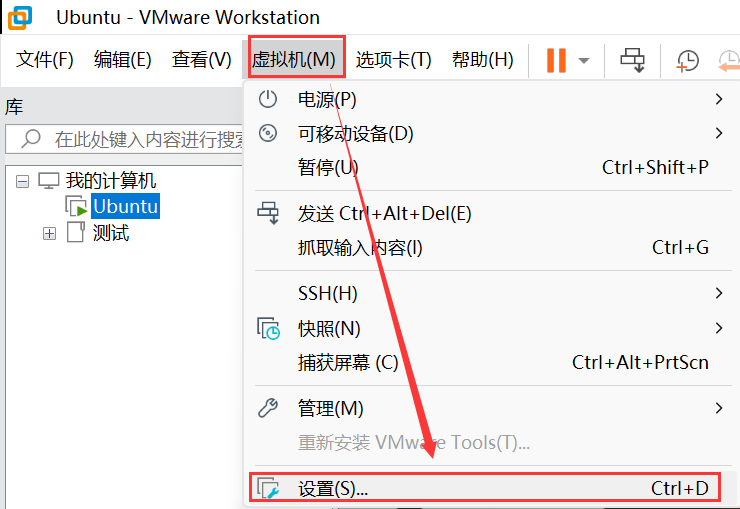
\includegraphics[width=\textwidth]{gxwjj-1.png}
    \end{subfigure}
    \hfill
    \begin{subfigure}[c]{0.35\textwidth}
      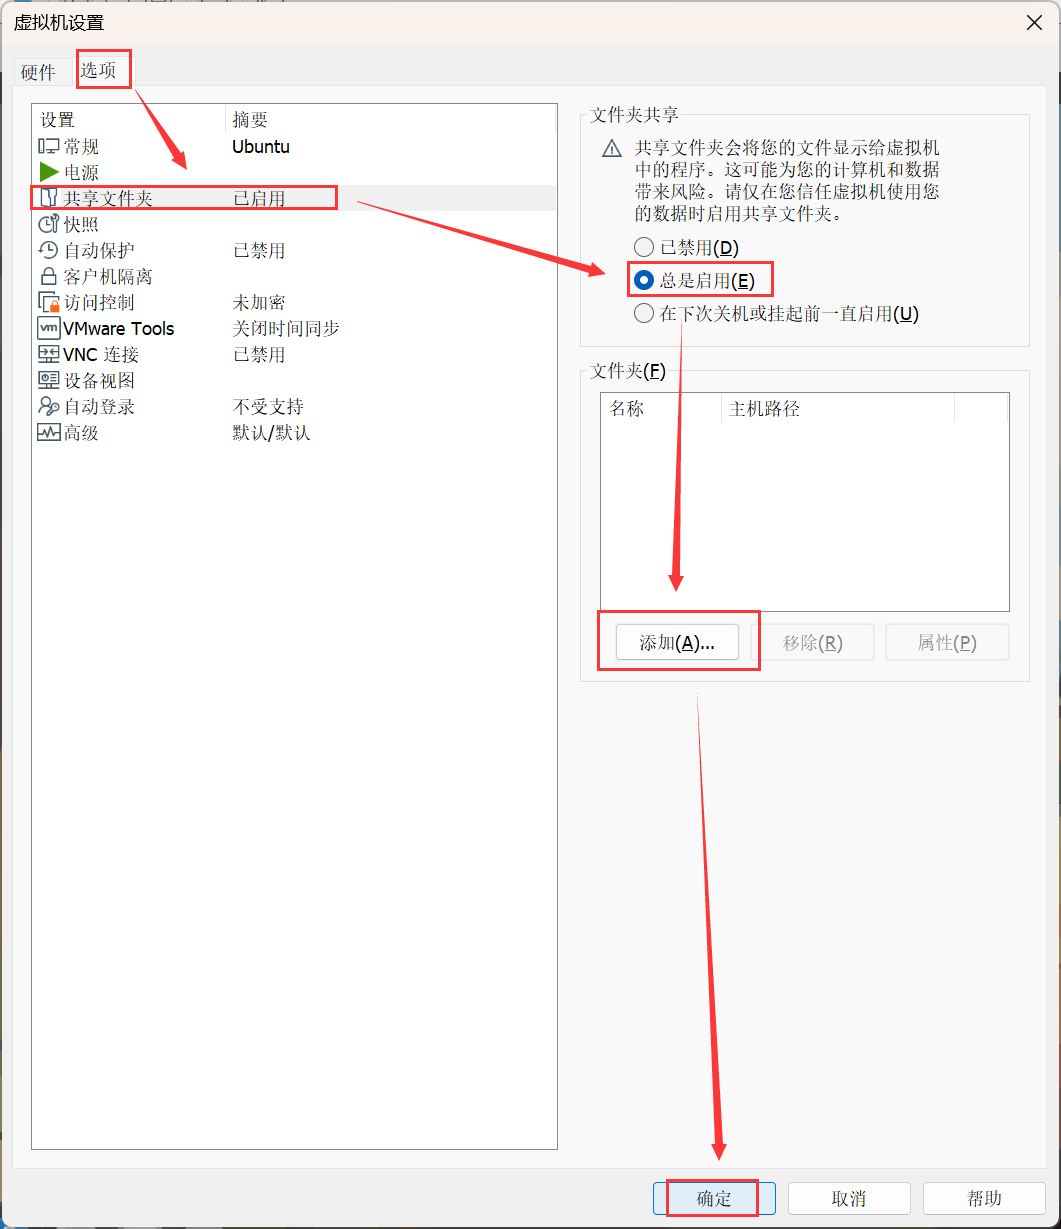
\includegraphics[width=\textwidth]{gxwjj-2.png}
    \end{subfigure}
    \caption{设置共享文件夹}
    \label{fig:shared-folder-setup}
\end{figure}

在“添加共享文件夹向导”的这一步时,点击“浏览”选择需要共享的文件夹,名称可不填:
\begin{figure}[h]
    \centering
    \captionsetup{font={small, bf}, margin=60pt}
    \begin{subfigure}[c]{0.5\textwidth}
    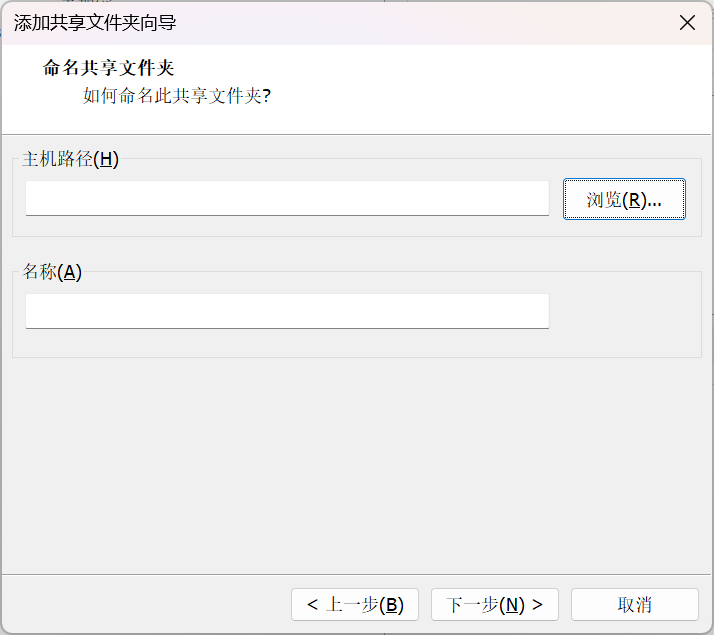
\includegraphics[width=\textwidth]{gxwjj-3.png}
    \end{subfigure}    
    \caption{共享文件夹向导}
    \label{fig:shared-folder-wizard}
\end{figure}

以上设置完成后,打开终端,运行以下命令:
\begin{envcode}{console}{Bash}
user1@host:~$ vmware-hgfsclient
\end{envcode}
若列出了所有共享的文件夹名称,则表示共享文件夹设置成功。

继续运行以下命令:
\begin{envcode}{console}{Bash}
user1@host:~$ sudo /usr/bin/vmhgfs-fuse .host:/ /mnt/hgfs -o allow_other -o uid=1000 -o gid=1000 -o umask=022
\end{envcode}
这将把共享文件夹挂载到`/mnt/hgfs`目录下。

现在,你可以通过以下命令访问共享文件夹:
\begin{envcode}{console}{Bash}
user1@host:~$ cd /mnt/hgfs
user1@host:/mnt/hgfs$ ls
SharedFolder1  SharedFolder2  ...
\end{envcode}
若显示了共享文件夹,则表示共享文件夹设置成功。

接下来设置开机自动挂载,
编辑`/etc/fstab`文件:
\begin{envcode}{console}{Bash}
user1@host:~$ sudo vim /etc/fstab
\end{envcode}

按“i”进入插入模式,移动光标到最后一行,
在文件末尾新建一行添加以下内容:
\begin{envcode}{text}{Text}
.host:/ /mnt/hgfs fuse.vmhgfs-fuse allow_other,uid=1000,gid=1000,umask=022 0 0
\end{envcode}

按“Esc”键退出插入模式,然后输入“:wq”后回车保存并退出。

重启虚拟机,进入/mnt/hgfs目录,如果可以看到共享的文件夹,则说明开机自动挂载设置成功。

如果需要访问共享文件夹,只需进入`/mnt/hgfs`目录即可。

如果之后需要添加新的共享文件夹,重复第一步,添加新的共享文件夹即可,不必重复设置开机自动挂载。
